\documentclass[aspectratio=43,10pt]{beamer}
\usecolortheme{default}
\setbeamertemplate{itemize items}[circle]
\setbeamertemplate{navigation symbols}{}
\setbeamertemplate{footline}[frame number]
\usepackage[T1]{fontenc}
\usepackage{lmodern}
\usepackage{booktabs,tabularx,array,xcolor}
\usepackage{tikz}
\usetikzlibrary{arrows.meta,positioning,fit,calc}
\definecolor{aggiemaroon}{RGB}{80,0,0}
\definecolor{deepblue}{RGB}{28,62,99}
\definecolor{teal}{RGB}{0,106,112}
\definecolor{pale}{RGB}{233,243,246}
\definecolor{risk}{RGB}{162,72,38}
\setbeamercolor{structure}{fg=aggiemaroon}
\setbeamercolor{block title}{bg=aggiemaroon,fg=white}
\setbeamercolor{block body}{bg=pale,fg=black}
\setbeamercolor{alerted text}{fg=risk}
\newcommand{\smallnote}[1]{\vspace{0.4em}{\scriptsize\color{gray}#1}}
\tikzset{stage/.style={draw=deepblue,very thick,rounded corners=3pt,fill=pale,align=center,text width=1.9cm,minimum height=0.90cm,font=\small}, link/.style={-{Latex[length=2.5mm]},thick,draw=teal}, dependency/.style={-{Latex[length=2mm]},thick,draw=risk,dashed}, labelnode/.style={font=\scriptsize,align=center}}
\title{Data Architecture:\\Examples, Tools, and Design Decisions}
\subtitle{Plan first, map dependencies, test assumptions, then implement!}
\author{}
\date{\textcolor{aggiemaroon}{DAEN 459 -- Fall 2026\\
      \textbf{Alexander Abuabara}}}
\titlegraphic{\vfill 
\includegraphics[height=1.2cm]{TAMU_logo.png}}

\begin{document}

\begin{frame}\titlepage\end{frame}

\begin{frame}{Outcomes}
\begin{enumerate}
\item Compare three common data architectures and the constraints that favor each.
\item Explain what each tool does and identify credible alternatives.
\item Use architecture maps, dependency graphs, and lineage diagrams to uncover risks.
\item Record decisions, assumptions, and tests \emph{before} building the entire pipeline.
\end{enumerate}
\begin{block}{Key message}A diagram is not just documentation:\\it is a planning and dependency-checking instrument.\end{block}
\end{frame}

\begin{frame}{Plan the system before choosing products}
\begin{columns}[T]
\column{.51\textwidth}
\textbf{Capture requirements}
\begin{itemize}
\item Consumers and expected outputs
\item Sources, ownership, formats, frequency
\item Freshness requirements: daily, hourly, seconds
\item Volume, growth, security, budget
\item Recovery and data-quality expectations
\end{itemize}
\column{.46\textwidth}
\textbf{Create planning artifacts}
\begin{enumerate}
\item Context diagram: systems and owners
\item Data flow: movement and storage
\item Dependency DAG: ordering and failure effects
\item Decision log: choices and alternatives
\item Thin vertical-slice test: one output end to end
\end{enumerate}
\end{columns}
\begin{block}{Planning question}What has to be true for this design to work? Show where those assumptions are verified.\end{block}
\end{frame}

\begin{frame}{A reusable architectural vocabulary}
\centering
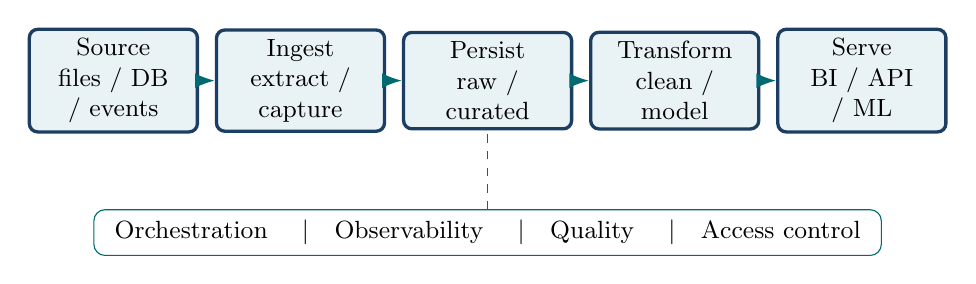
\begin{tikzpicture}[node distance=.2cm]
\node[stage] (s) {Source\\files / DB / events};
\node[stage,right=of s] (i) {Ingest\\extract / capture};
\node[stage,right=of i] (r) {Persist\\raw / curated};
\node[stage,right=of r] (t) {Transform\\clean / model};
\node[stage,right=of t] (o) {Serve\\BI / API / ML};
\foreach \a/\b in {s/i,i/r,r/t,t/o}{\draw[link] (\a)--(\b);}
\node[draw=teal,rounded corners,fill=white,minimum width=10cm,minimum height=.58cm,below=1.0cm of r,font=\small] (ops) {Orchestration  \quad\textbar\quad Observability \quad\textbar\quad Quality \quad\textbar\quad Access control};
\draw[dashed,teal] (ops.north)--(r.south);
\end{tikzpicture}
\vspace{.5em}
\begin{itemize}
\item Separate \textbf{logical design} (required capabilities) from \textbf{physical design} (specific tools).
\item Draw \textbf{data movement} and \textbf{control dependencies} separately when helpful.
\item Every arrow implies a contract: schema, format, schedule, authentication, or reliability.
\end{itemize}
\end{frame}

\begin{frame}{Example 1: Scheduled operational analytics (batch ELT)}
\textbf{Scenario:} A campus unit combines transactional database data and CSV exports into a daily dashboard.
\vspace{.6em}
\centering
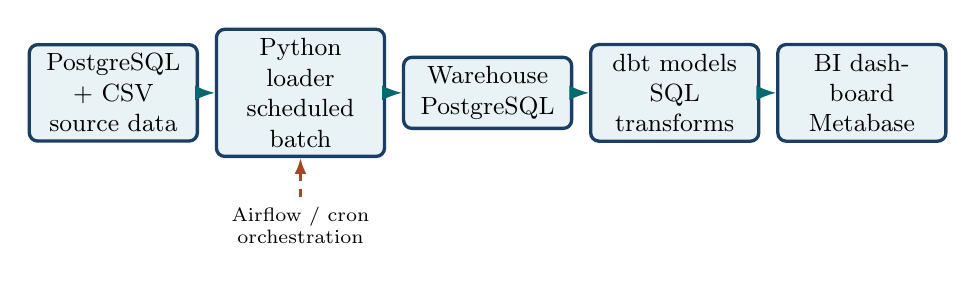
\begin{tikzpicture}[node distance=.2cm]
\node[stage] (src) {PostgreSQL + CSV\\source data};
\node[stage,right=of src] (load) {Python loader\\scheduled batch};
\node[stage,right=of load] (wh) {Warehouse\\PostgreSQL};
\node[stage,right=of wh] (dbt) {dbt models\\SQL transforms};
\node[stage,right=of dbt] (bi) {BI dashboard\\Metabase};
\foreach \a/\b in {src/load,load/wh,wh/dbt,dbt/bi}{\draw[link] (\a)--(\b);}
\node[labelnode,below=.5cm of load] (schedule) {Airflow / cron\\orchestration};
\draw[dependency] (schedule.north)--(load.south);
\end{tikzpicture}
\vspace{-1em}
\begin{columns}[T]
\column{.52\textwidth}\textbf{Why this architecture?}
\begin{itemize}\item Dashboard can tolerate daily freshness.\item SQL-centric transformations are auditable.\item Moderate scale supports a simple stack.\end{itemize}
\column{.45\textwidth}\textbf{Critical dependencies}
\begin{itemize}\item CSV delivery before ingestion\item Loader success before dbt run\item Tests pass before dashboard refresh\end{itemize}
\end{columns}
\end{frame}

\begin{frame}{Example 1: Tool choices and alternatives}
\small
\begin{tabularx}{\textwidth}{@{}p{2.1cm}p{3.0cm}X@{}}\toprule
Function & Example tool & Alternatives and decision trigger \\ \midrule
Ingestion & Python + SQL drivers & Airbyte for many connectors; managed ingestion if operations are constrained \\
Storage & PostgreSQL & DuckDB for single-machine analysis; BigQuery/Snowflake for cloud-scale multi-user workloads \\
Transforms & dbt (SQL) & Python/Pandas for custom code; Spark for distributed processing \\
Scheduling & cron or Airflow & Prefect/Dagster for richer workflows; cron if dependencies are trivial \\
Serving & Metabase & Power BI, Tableau, or custom application \\
\bottomrule\end{tabularx}
\vspace{.6em}
\begin{block}{Decision}Choose the \textbf{smallest manageable stack} that meets correctness, freshness, and maintainability needs. Airflow is not necessary for one independent daily script.\end{block}
\end{frame}

\begin{frame}{Example 1: Dependency map exposes failures}
\centering
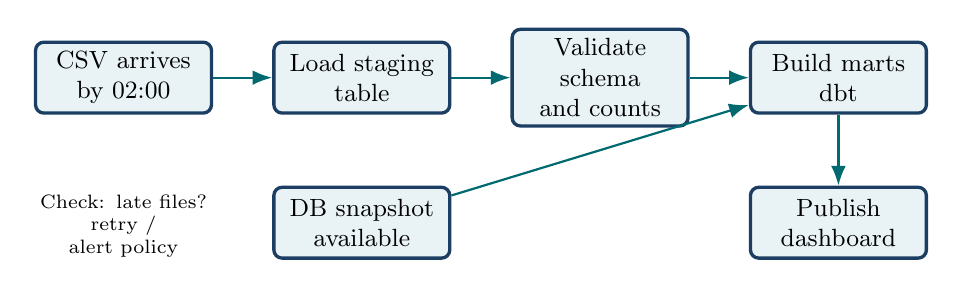
\begin{tikzpicture}[node distance=1.0cm and .75cm]
\node[stage,text width=2.0cm] (a) {CSV arrives\\by 02:00};
\node[stage,right=of a,text width=2.0cm] (b) {Load staging\\table};
\node[stage,right=of b,text width=2.0cm] (c) {Validate schema\\and counts};
\node[stage,right=of c,text width=2.0cm] (d) {Build marts\\dbt};
\node[stage,below=.9cm of d,text width=2.0cm] (e) {Publish\\dashboard};
\node[stage,below=.9cm of b,text width=2.0cm] (f) {DB snapshot\\available};
\foreach \x/\y in {a/b,b/c,c/d,d/e,f/d}{\draw[link] (\x)--(\y);}
\node[labelnode,below=.9cm of a,text width=2.2cm] {Check: late files?\\retry / alert policy};
\end{tikzpicture}
\vspace{.5em}
\begin{itemize}
\item The DAG shows \textbf{execution dependencies}, not just data movement.
\item Identify gates: expected source arrival, schema tests, row-count checks.
\item Define actions for late files, changed columns, and partial loads.
\end{itemize}
\end{frame}

\begin{frame}{Example 2: API + object storage + analytical processing}
\textbf{Scenario:} A research team ingests external API data and documents, preserves raw versions, and prepares reproducible datasets.
\vspace{.5em}
\centering
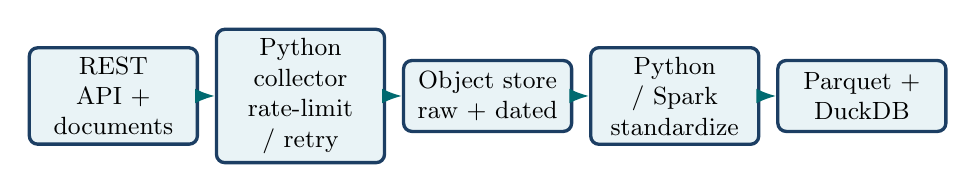
\begin{tikzpicture}[node distance=.2cm]
\node[stage] (a) {REST API +\\documents};
\node[stage,right=of a] (b) {Python collector\\rate-limit / retry};
\node[stage,right=of b] (c) {Object store\\raw + dated};
\node[stage,right=of c] (d) {Python / Spark\\standardize};
\node[stage,right=of d] (e) {Parquet +\\DuckDB};
\foreach \x/\y in {a/b,b/c,c/d,d/e}{\draw[link] (\x)--(\y);}
\end{tikzpicture}
\vspace{-1em}
\begin{columns}[T]
\column{.49\textwidth}\textbf{Architecture rationale}
\begin{itemize}\item Raw snapshots enable replay and auditing.\item Columnar files support repeatable analysis.\item Collection and processing can scale separately.\end{itemize}
\column{.48\textwidth}\textbf{Planning checks}
\begin{itemize}\item API quotas and schema drift\item File naming/partition conventions\item Credentials, access and retention\item Reprocessing when logic changes\end{itemize}
\end{columns}
\end{frame}

\begin{frame}{Example 2: Alternatives and trade-offs}
\small
\begin{tabularx}{\textwidth}{@{}p{2.2cm}p{3.2cm}X@{}}\toprule
Decision & Option A & Option B / selection evidence \\ \midrule
Raw storage & Local files / NAS & S3 / Azure Blob / GCS: shared scalable storage, with cloud costs and access setup \\
Compute & Python / Polars / DuckDB & Spark: distributed work when one machine no longer meets measured targets \\
Curated format & Parquet files & Database tables: concurrency / updates / serving requirements may favor tables \\
Orchestration & Scheduled Python jobs & Prefect / Airflow / Dagster if retries, backfills, and dependencies grow \\
\bottomrule\end{tabularx}
\vspace{-1em}
\begin{block}{Decision evidence}Benchmark a representative dataset; document API limits, storage footprint, query time, reprocessing time, and access controls.\end{block}
\end{frame}

\begin{frame}{Example 2: Map upstream and downstream dependencies}
\centering
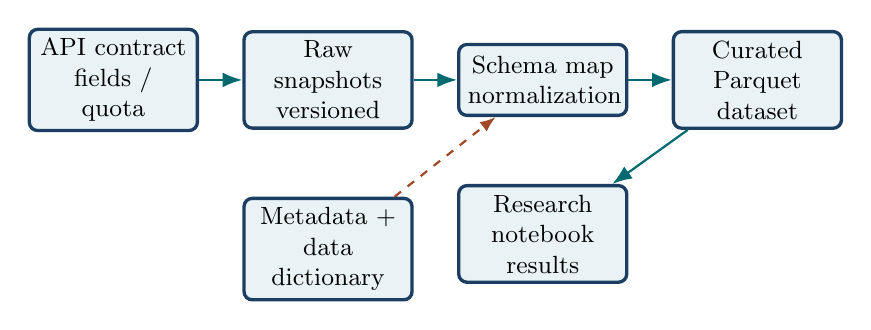
\begin{tikzpicture}[node distance=.7cm and .55cm]
\node[stage] (api) {API contract\\fields / quota};
\node[stage,right=of api] (raw) {Raw snapshots\\versioned};
\node[stage,right=of raw] (schema) {Schema map\\normalization};
\node[stage,right=of schema] (clean) {Curated Parquet\\dataset};
\node[stage,below=.85cm of schema] (notebook) {Research notebook\\results};
\foreach \x/\y in {api/raw,raw/schema,schema/clean,clean/notebook}{\draw[link] (\x)--(\y);}
\node[stage,below=.85cm of raw] (dict) {Metadata +\\data dictionary};
\draw[dependency] (dict)--(schema);
\end{tikzpicture}
\vspace{.6em}
\begin{itemize}
\item \textbf{Impact question:} If an API field changes, which curated columns and analyses break?
\item Maintain a source-to-target mapping and document schema assumptions.
\item Check whether full rebuilds are possible using saved raw data.
\end{itemize}
\end{frame}

\begin{frame}{Example 3: Event-driven near-real-time monitoring}
\textbf{Scenario:} IoT devices send measurements; the system detects abnormal conditions and exposes recent aggregates within seconds/minutes.
\vspace{.4em}
\centering
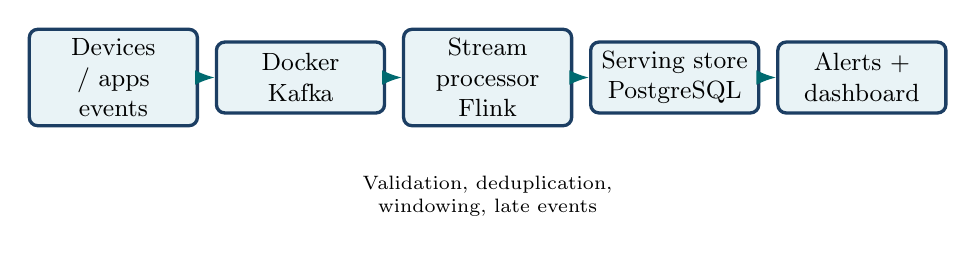
\begin{tikzpicture}[node distance=.2cm]
\node[stage] (a) {Devices / apps\\events};
\node[stage,right=of a] (b) {Docker\\Kafka};
\node[stage,right=of b] (c) {Stream processor\\Flink};
\node[stage,right=of c] (d) {Serving store\\PostgreSQL};
\node[stage,right=of d] (e) {Alerts +\\dashboard};
\foreach \x/\y in {a/b,b/c,c/d,d/e}{\draw[link] (\x)--(\y);}
\node[labelnode,below=.5cm of c] {Validation, deduplication,\\windowing, late events};
\end{tikzpicture}
\vspace{-1em}
\begin{columns}[T]
\column{.50\textwidth}\textbf{Rationale}
\begin{itemize}\item Events arrive continuously.\item Processing must handle delays and duplicates.\item Broker decouples producers and consumers.\end{itemize}
\column{.47\textwidth}\textbf{Dependencies to map}
\begin{itemize}\item Event schema / device identity\item Broker health and retention\item Processor state / checkpointing\item Downstream alert availability\end{itemize}
\end{columns}
\end{frame}

\begin{frame}{Example 3: Is streaming actually necessary?}
\small
\begin{tabularx}{\textwidth}{@{}p{2.3cm}p{3.0cm}X@{}}\toprule
Requirement & Simpler path & Streaming path \\ \midrule
Freshness & Poll API / micro-batch every few minutes & Continuous Kafka + Flink when low latency is a measured requirement \\
Data movement & Direct write to DB / queue & Durable event broker for decoupling, replay, multiple consumers \\
Compute & Python worker / scheduled SQL & Stream processing for stateful windows, out-of-order events \\
Operations & Few services, simpler debugging & More components, deployments, monitoring, and recovery modes \\
\bottomrule\end{tabularx}
\vspace{.7em}
\begin{block}{Decision}Prototype polling first if the project can tolerate minutes of delay. Only adopt Kafka/Flink when measured latency, replay, or scale needs justify operating them.\end{block}
\end{frame}

\begin{frame}{Compare the three designs}
\small
\begin{tabularx}{\textwidth}{@{}p{2.55cm}XXX@{}}\toprule
Dimension & Batch warehouse & API + lake files & Event-driven streaming \\ \midrule
Typical cadence & Daily / hourly & Periodic / on demand & Continuous \\
Main asset & Curated relational marts & Replayable raw snapshots + curated datasets & Durable event flow + current state \\
Biggest concern & Scheduling and stale data & API contracts and reproducibility & Ordering, duplicates, latency, operations \\
Good initial test & One full daily refresh & Ingest, store, and replay one partition & Simulate bursts and late events \\
Avoid by default & Excessive orchestration & Distributed compute too early & Complex brokers without an SLA \\
\bottomrule\end{tabularx}
\vspace{.7em}
\par\textbf{No architecture is ``best'' in isolation:} the requirements and dependency risks determine the choice.
\end{frame}

\begin{frame}{Four complementary maps teams should maintain}
\begin{enumerate}
\item \textbf{System context:} upstream providers, users, organizational boundaries, credentials.
\item \textbf{Data flow / lineage:} datasets and fields, transforms, materializations, consumers.
\item \textbf{Execution dependency DAG:} scheduling, prerequisites, retries, backfills, stop/go quality gates.
\item \textbf{Deployment and service map:} packages, databases, endpoints, secrets, environments, owners.
\end{enumerate}
\begin{block}{Suggested tools}
\textbf{Diagramming:} draw.io/diagrams.net, Mermaid, Graphviz.\\
\textbf{Workflow DAGs:} Airflow, Dagster, Prefect.\\
\textbf{Data lineage:} dbt docs, OpenLineage/Marquez, catalog tools.\\
\textbf{Code/package dependencies:} pipdeptree, \texttt{uv tree}, dependency lockfiles, CI checks.
\end{block}
\par\smallnote{Choose tools based on project scope; a well-maintained diagram is better than an elaborate unused platform.}
\end{frame}

\begin{frame}{How to audit a dependency map}
\begin{columns}[T]
\column{.50\textwidth}
\textbf{For each node, annotate:}
\begin{itemize}
\item Owner and environment
\item Input / output contract and schema
\item Trigger and expected completion time
\item Failure detection / retry policy
\item Security classification and access
\item Downstream consumers and SLA
\end{itemize}
\column{.47\textwidth}
\textbf{Then challenge the edges:}
\begin{itemize}
\item Missing prerequisite or circular dependency?
\item Single point of failure?
\item What changes if a schema version changes?
\item Can this step be repeated safely?
\item What is the blast radius of failure?
\item Can data be replayed or backfilled?
\end{itemize}
\end{columns}
\begin{block}{Practical review}Walk one normal record and one failed/late record through the entire diagram.\end{block}
\end{frame}

\begin{frame}{Tool-selection matrix: score evidence, not enthusiasm}
\small
\begin{tabularx}{\textwidth}{@{}p{3.0cm}cXX@{}}\toprule
Criterion & Weight & Option A: simple batch & Option B: streaming stack \\ \midrule
Meets freshness goal & 30\% & 3 / 5 & 5 / 5 \\
Implementation effort & 25\% & 5 / 5 & 2 / 5 \\
Operational burden & 20\% & 5 / 5 & 2 / 5 \\
Scalability headroom & 15\% & 3 / 5 & 5 / 5 \\
Team familiarity & 10\% & 5 / 5 & 2 / 5 \\ \midrule
Illustrative weighted score & 100\% & \textbf{4.10 / 5} & \textbf{3.15 / 5} \\ \bottomrule
\end{tabularx}
\vspace{.5em}
\begin{itemize}
\item Scores are \textbf{illustrative}, not product facts; derive real scores from prototypes.
\item Apply hard constraints (e.g., must meet a 5-second SLA) \textbf{before} ranking options.
\item Record sensitivity: would the recommendation change if a weight doubled?
\end{itemize}
\end{frame}

\begin{frame}{Architecture Decision Record (ADR): one decision per page}
\begin{block}{Example: ADR-003 --- batch vs. streaming ingestion}
\textbf{Context:} dashboard stakeholders can accept 10-minute freshness.\\
\textbf{Options:} (A) scheduled API poll + database; (B) Kafka + stream processor.\\
\textbf{Decision:} prototype A as baseline.\\
\textbf{Why:} lower operational complexity; requirement currently permits polling.\\
\textbf{Risks:} rate limits, missed updates, API outages.\\
\textbf{Validation:} replay test + 95th-percentile end-to-end freshness.\\
\textbf{Revisit if:} requirements tighten or polling cannot meet reliability goals.
\end{block}
\smallnote{An ADR captures context, alternatives, consequences, evidence, and the conditions for revisiting the choice.}
\end{frame}

\begin{frame}{Capstone work plan: artifacts before a full build}
\small
\begin{tabularx}{\textwidth}{@{}p{2.1cm}X p{4.2cm}@{}}\toprule
Phase & Team action & Evidence / deliverable \\ \midrule
1. Define & Describe use case and measurable constraints & One-page requirement / acceptance criteria \\
2. Map & Sketch logical architecture and four dependency views & Versioned diagrams, assumptions list \\
3. Compare & Select 2--3 credible architecture/tool options & Decision matrix + preliminary ADR \\
4. Probe & Implement one end-to-end vertical slice & Timing, cost, quality, recovery test \\
5. Refine & Review dependencies and failure paths & Updated maps, revised ADR, backlog \\
\bottomrule\end{tabularx}
\vspace{.65em}
\begin{block}{Do not start with an installation sprint}First find the riskiest unverified assumption, then design a small experiment that can invalidate it.\end{block}
\end{frame}

\begin{frame}{In-class capstone exercise (20--25 minutes)}
\begin{enumerate}
\item \textbf{5 min:} Draw sources, ingestion, storage, transformation, and consumers.
\item \textbf{5 min:} Add arrows for execution dependencies and mark at least three possible failure points.
\item \textbf{5 min:} Identify one simpler and one more sophisticated tool alternative.
\item \textbf{5 min:} Draft an ADR with a single falsifiable decision criterion.
\item \textbf{5 min:} Exchange maps with another team; have them find missing dependencies.
\end{enumerate}
\begin{block}{Share-out prompt}What dependency or hidden assumption did your map reveal, and what evidence would change your tool choice?\end{block}
\end{frame}

\begin{frame}{What the team should leave with}
\begin{itemize}
\item One \textbf{clear architecture map} with meaningful component and data-flow labels.
\item One \textbf{dependency DAG} showing ordering, quality gates, and failure handling.
\item Two or three \textbf{credible tool/architecture alternatives} evaluated against requirements.
\item An \textbf{ADR} with a decision, trade-offs, and revisit conditions.
\item A \textbf{small experiment} to validate the highest-risk assumption.
\end{itemize}
\vspace{.6em}
\centering\Large\textbf{Plan $\rightarrow$ Map $\rightarrow$ Challenge $\rightarrow$ Test $\rightarrow$ Decide}
\end{frame}

\end{document}